% Foliensatz: "AFu-Kurs nach DJ4UF" von DK0TU, Amateurfunkgruppe der TU Berlin
% Lizenz: CC BY-NC-SA 3.0 de (http://creativecommons.org/licenses/by-nc-sa/3.0/de/)
% Autoren: Martin Deutschmann

preamble.dk0tu.tex
\subtitle{Technik Klasse A 10: \\
          HF-Leitungen \& Kabel \\[2em]}
\date{Stand 01.06.2015}
 \begin{document}

\begin{frame}
    \titlepage
    \vfill
    \begin{center}
        \ccbyncsaeu\\
        {\tiny This work is licensed under the \em{Creative Commons Attribution-NonCommercial-ShareAlike 3.0 License}.}\\[0.5ex]
         \tiny Amateurfunkgruppe der Technische Universität Berlin (AfuTUB), DKØTU
         %\includegraphics[scale=0.5]{img/DK0TU_Logo.pdf}
    \end{center}
\end{frame}


%fixme Referenzen/Fußnoten-Systematik vereinheitlichen

\section*{Hochfrequenzleitung}
\begin{frame}
\frametitle{Hochfrequenzleitungen}
\begin{center}
%\begin{minipage}{0.4\textwidth}
\includegraphics[scale=0.25]{a10/parallel.png}\\
Abb.1: Paralleldrahtleitung \cite{wp}
%\end{minipage}\\
\\
%\begin{minipage}{0.4\textwidth}
\includegraphics[scale=0.4]{a10/coax.png}\\
Abb.2: Koaxialkabel \cite{wm}
%\end{minipage}
\end{center}
\end{frame}

\begin{frame}
\frametitle{Hochfrequenzleitungen}
\begin{center}
\includegraphics[scale=0.4]{a10/hohl.jpg}\\
Abb.3: Hohlleiter \cite{wp}
%\end{minipage}
\end{center}
\end{frame}

\section*{Wellenwiderstand}
\begin{frame}
\frametitle{Wellenwiderstand}
\includegraphics[scale=0.8]{a10/wellenesb.png}\\
Abb.4: ESB 
\vspace{1cm}\\
\includegraphics[scale=0.65]{a10/wellenesbex.png}\\
Abb.5: Genaues Ersatzschaltbild eines Koxialkabels
\end{frame}

\begin{frame}
\frametitle{Wellenwiderstand}
\begin{itemize}
	\item \Huge{ $Z_W = \sqrt{\frac{L'}{C'}}$}
	 \normalsize \item Paralleldrahtleitungen: Zw = 150 $\Omega$ bis 600 $\Omega$
	\item Koaxialleitungen: Zw =  50 $\Omega$ bis 95 $\Omega$
	\item Der Wellenwiderstand entspricht dem Abschlusswiderstand einer Leitung, bei dem keine stehenden Wellen auftreten.
\end{itemize}
\end{frame}

\section*{Der Verkürzungsfaktor}
\begin{frame}
\frametitle{der Verkürzungsfaktor}
\begin{itemize}
	\item	Das Dielektrikum verlangsamt die Ausbreitungsgeschwindigkeit im Kabel
	\item	Ausbreitungsgeschwindigkeit wird wie folgt berechnet:
	\begin{LARGE}
	\item	$v = \frac{1}{\sqrt{L' C'}}$
	\end{LARGE}	
	\item	Durch geringere Ausbreitungsgeschwindigkeit verkürzt sich die Wellenlänge  auf der Leitung
	\begin{LARGE}
	\item	$k = \frac{v}{c}$ 
	\end{LARGE}
\end{itemize}
\end{frame}

\begin{frame}
\frametitle{Typische Verkürzungsfaktoren}
\begin{center}
\begin{tabular}{|l|l|}
	\hline
	Koaxialkabel, normal & $k = 0,66$ \\ \hline
	Koaxialkabel mit Luftisolation & $k = 0,85$ \\ \hline
	offene $600 \Omega$ Speiseleitung & $k = 0,98$ \\ \hline
	Flachleitung mit $300 \Omega$ & $k = 0,82$ \\ \hline
\end{tabular}
\end{center}
\end{frame}

\section*{Die D\"ampfung}
\begin{frame}
\frametitle{Die Dämpfung}
\begin{itemize}
	\item	Gibt den Leistungsverlust über das Kabel an
	\item	Hängt vom Verlustwiderstand und dem Dielektrikum ab
	\item	Wird meist in dB pro $100m$ angegeben
	\begin{Large}
	\item	$n = \sqrt{\frac{f_{hoch}}{f_{niedrig}}}$
	\end{Large}	
\end{itemize}
\end{frame}

\begin{frame}
\frametitle{ein kleines Beispiel}
	Beispiel: RG 213/U hat bei $100MHz$ eine Dämpfung von $6,7dB$. Wie groß ist die Dämpfung bei $145MHz$?
	\vspace{1cm}
	\begin{Large}
	$n = \sqrt{\frac{f_2}{f_1}} = \sqrt{\frac{145}{100}} = \sqrt{1,45} = 1,2$
	\end{Large}
	\vspace{1cm}
	Bei $145MHz$ ist die Dämpfung also: \\
	$1,2 \cdot 6,7dB = 8dB$
\end{frame}

\begin{frame}
\frametitle{D\"ampfungsberechnung}
\begin{Large}
Ich hoffe ihr habt eure Formelsammlung dabei C:
\end{Large}
\end{frame}

\begin{frame}
\frametitle{Let's calculate together}
\begin{minipage}{0.3\textwidth}
\begin{itemize}
 	\item RG58\\
 	\item 15 m\\
 	\item 28 MHz
 \end{itemize}
\end{minipage}
\begin{minipage}{0.3\textwidth}
\begin{itemize}
 	\item Aircell7\\
 	\item 15 m\\
 	\item 28 MHz
 \end{itemize}
\end{minipage}
\begin{minipage}{0.3\textwidth}
\begin{itemize}
 	\item RG174\\
 	\item 15 m\\
 	\item 28 MHz
 \end{itemize}
\end{minipage}
\end{frame}

\section*{Stehwellenverh\"altnis}
\begin{frame}
\frametitle{Stehwellenverh\"altnis}
\begin{itemize}
	\item ist ein Maß für die Anpassung
	\begin{Large}
	\item	$SWR = s = \frac{U_{max}}{U_{min}}$
	\end{Large}
	\item	hängt direkt vom Verhältnis Abschlusswiderstand $R_a$ zu Wellenwiderstand $Z_W$ ab
	\vspace{2mm}
	\begin{Large}
	\item	$SWR = s = \frac{U_{max}}{U_{min}} = \frac{Z}{R_a} $für$ R_a \geq Z$
	\vspace{2mm}
	\item	$SWR = s = \frac{U_{max}}{U_{min}} = \frac{R_a}{Z} $für$ Z \geq R_a$
	\end{Large}
	\vspace{2mm}
	\item ist das Verhältnis von vorlaufender zu zurücklaufender Welle
	\item \url{http://commons.wikimedia.org/wiki/File:Stehwelle_(Animation).gif}
\end{itemize}
\end{frame}

\section*{Die Lecherleitung}
\begin{frame}
\frametitle{Die Lecherleitung}
\begin{center}
\includegraphics[scale=0.25]{a10/Lecherkreis.png}\\
Abb.6: Lecherkreis
\end{center}
\begin{itemize}
	\item	Ist ein Sonderfall einer Transformationsleitung mit einem Absclusswiderstand von $0 \Omega$ oder $\infty \Omega$
	\item	 Gibt man HF-Signal auf Doppelleitung, mit $R_a = 0 \Omega$ wird die gesamte Energie reflektiert
	\item	Dadurch entstehen Auslöschungen und Anhebungen
	\item	Wellenwiderstand kehrt sich alle $\lambda /4$ um
	\item	Lässt man das Leitungsende offen, kehren sich alle Verhältnisse um
	\item	Dieser Effekt tritt auch bei einer $\lambda /2$ Leitung auf
\end{itemize} 
\end{frame}

\begin{frame}
\frametitle{Die Lecherleitung}
\begin{Large}
\begin{itemize}
	\item	Zusammenfassung:
	\vspace{1cm}
	\item	$\lambda /4$ Leitung kehrt Impedanzverhältnisse um(niederohmig -hochohmig), wirkt wie Schwingkreis
	\vspace{1cm}
	\item	$\lambda /2$ Leitung transformiert 1:1, wirkt auch wie ein Schwingkreis
\end{itemize}
\end{Large}
\end{frame}

\section*{Transformationsleitungen}
\begin{frame}
\frametitle{Transformationsleitungen}
\begin{itemize}
	\item	Dienen der Anpassung von Antenne zum Sender
	\item	Dafür wird zum einen der Widerstand des Senders an die HF-Leitung
	\item	Und andererseits die Antennenimpedanz an das Kabel angepasst
	\begin{Large}
	\item	$R_i = Z_w = Z_{Antenne}$
	\end{Large}
\end{itemize}
\end{frame}

\begin{frame}
\frametitle{Prinzip der Tranformationsleitung}
	\includegraphics[scale=0.5]{a10/Anpassung.png}\\
	Abb.7: Anpassung \cite{wp}
	\begin{itemize}
		\item	Eine $\lambda /4$-Leitung kann Widerstände tranformieren
		\item	Aber nur, in einer begrenzten Bandbreite
		\item	Leitung wirkt als Transformator
		\item	Eine solche Leitung bestimmter Länge auch als abgestimmte Speiseleitung bezeichnet
		\item	Leitungen die mit ihrem Wellenwiderstand abgeschlossen werden, um Stehwellen zu vermeiden, nennt man unabgestimmte Speiseleitung
	\end{itemize}
\end{frame}

\begin{frame}
\begin{itemize}
	\item	Will man zwei Impedanzen $Z_2$ \& $Z_2$ anpassen, so muss die Transformationsleitung folgende Werte besitzen:
	\item	Wellenwiderstand:\\ 
	\vspace{2mm}
	\begin{Large}	
	$Z = \sqrt{Z_1 \cdot Z_2}$
	\end{Large}
	\vspace{2mm}
	\item	Länge: \\ 
	\vspace{2mm}
	\begin{Large}
	$l = (2n - 1) \cdot \frac{\lambda}{4} \cdot k$
	\end{Large}
	\vspace{3mm}
	\item	Bei Koaxialkabeln sieht das Ganze wie folgt aus:
	\vspace{3mm}
	\begin{Large}
		$z = \frac{138 \Omega}{\sqrt{\varepsilon_r}} \cdot lg(\frac{D}{d})$
	\end{Large}		
\end{itemize}
\end{frame}

\section*{Symmetrierung}
\begin{frame}
\frametitle{Symmetrierung}
\begin{minipage}{0.3\textwidth}
	\includegraphics[scale=0.5]{a10/balun.jpg}\\
	Abb.8: Balun \cite{wp}
\end{minipage}	
\hspace{2mm}
\begin{minipage}{0.5\textwidth}
	\begin{itemize}
		\item Wird bei Verbindungen zwischen symmetrischen und unsymmetrischen Punkten verwendet
		\item Koaxialkabel ist unsymmetrisch
		\item Paralleldraht ist symmetrisch
		\item Alle Dipole sind symmetrisch
		\item Alle Antennen die gegen Erde erregt werden sind unsymmetrisch
		\item	Ohne Symmetrierung entstehen Mantelwellen
	\end{itemize}
\end{minipage}
\end{frame}

\begin{frame}
\frametitle{Balun}
\includegraphics[scale=0.5]{a10/balun.png}\\
Abb.9: Spartrafo als Balun \cite{wm}
\begin{itemize}
	\item	Balun kann symmetrieren und gleichzeitig die Impedanz anpassen
	\item	Wird der Eingang an halber Windungszahl des Ausganges angeschlossen, erhält man einen 1:4 Übertrager 
\end{itemize}	
\end{frame}

\begin{frame}
\frametitle{Die $\lambda /2$-Umwegleitung}
\begin{minipage}{0.3\textwidth}
	\includegraphics[scale=0.3]{a10/Umwegleitung.jpg}\\
	Abb.10: $\lambda /2$-Umwegleitung \cite{wp}
\end{minipage}	
\hspace{2mm}
\begin{minipage}{0.5\textwidth}
	\begin{footnotesize}
	\begin{itemize}
		\item	An der Einspeisestelle teilt sich der Strom je zur Hälfte auf
		\item	Eine Hälfte geht direkt zum Strom, die andere in die Umwegleitung
		\item	Nach dem ohmschen Gesetz verdoppelt sich dadurch der Widerstand
		\item	Bei $50 \Omega$ ergeben sich also $100 \Omega$ 
		\item	Die Umwegleitung stellt den Widerstand auf der anderen Seite nochmal mit $100 \Omega$ zur Verfügung
		\item	Somit ergeben sich insgesamt $200 \Omega$ Impedanz an der Antenne
	\end{itemize}
	\end{footnotesize}
\end{minipage}
\end{frame}

\section*{Der Topfkreis}
\begin{frame}
\frametitle{Der Topfkreis}
\begin{center}
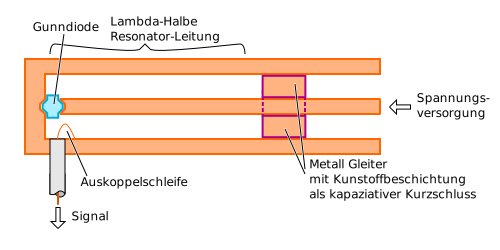
\includegraphics[scale=0.2]{a10/Topfkreis.png}
\hspace{2mm}
\includegraphics[scale=0.8]{a10/Topfkreis-ESB.png}\\
Abb.11: Topfkreis und ESB
\end{center}
\begin{tiny}
\begin{itemize}
	\item	Im UHF-Bereich werden auch Aluminium- oder versilberte Messingbecher als Leiter genutzt
	\item	Sie besitzen einen Mittelleiter, wodurch sie wie eine Koaxleitung wirken
	\item	Sie lassen sich wie auch die Lecherleitung durch einen Kurzschlussschieber abstimmen
	\item	Dieser Schwingkreis ist vollkommen abgestimmt und von außen nicht beeinflussbar
	\item	Versilbert man die Innenflächen, lassen sich die Verlust minimieren
	\item	Dadurch werden auch die elektrischen Eigenschaften für hohe Frequenzen verbessert
\end{itemize}
\end{tiny}
\end{frame}

\renewcommand{\refname}{Referenzen}

\hypertarget{refs}{}
\textcolor{white}{} \\ %\vspace{} geht nicht
\Large Referenzen/Links
\footnotesize

\begin{thebibliography}{}
    \bibitem{darc}  DARC Online-Lehrgang Lektion A08:
                    \url{http://www.darc.de/referate/ajw/ausbildung/darc-online-lehrgang/technik-klasse-a/technik-a10/}
    
    \bibitem{wm} 	Wikimedia:
                    \url{http://commons.wikimedia.org/wiki/File:Coaxial_cable_cutaway_new.svg}
                    \url{http://commons.wikimedia.org/wiki/File:Cdbalun2.svg}
                        
    \bibitem{wp}    Wikipedia - Die freie Enzyklopädie:
                    \url{http://de.wikipedia.org/wiki/Datei:Twin-lead_cable_dimension.svg}
					\url{http://de.wikipedia.org/wiki/Datei:Elli_holl.jpg}
					\url{http://de.wikipedia.org/wiki/Datei:EingangswiderstandAusgangswiderstandA.svg}
					\url{http://de.wikipedia.org/wiki/Datei:Topfkreis_filter.svg}
					\url{http://de.wikipedia.org/wiki/Datei:EingangswiderstandAusgangswiderstandA.svg}
					\url{http://de.wikipedia.org/wiki/Datei:T200A2.jpg}
					\url{http://de.wikipedia.org/wiki/Datei:Balun(semirigid).jpg}

									
	\bibitem{bna}   Fragenkatalog Bundesnetzargentur Technik Klasse A:                   
                    \url{https://www.bundesnetzagentur.de/SharedDocs/Downloads/DE/Sachgebiete/Telekommunikation/Unternehmen_Institutionen/Frequenzen/Amateurfunk/Fragenkatalog/TechnikFragenkatalogKlasseAf252rId9014pdf.pdf?__blob=publicationFile&v=3}
\end{thebibliography} 

% Hier könnte noch eine Kontaktfolie stehen

\end{document}

